\section{実験} \label{section:evaluation}
提案方式によるヒュージページ割り当てとヒュージページなし,標準のヒュージページ割り当て(全体割り当て),
予備実験での手法でのヒュージページ割り当てと4つのヒュージページ割り当ての方法の4つのヒュージページ割り当てポリシーで実験を行った.
実験では実行時間やヒュージページ割り当てサイズ,TLBミス率などを計測した.TLBミスの計測にはperf\cite{perf}コマンドを用いている.
実験には作成した単純なマイクロベンチマークを利用した.マイクロベンチマークはStorageMemoryにデータをキャッシュし
そのデータに対してアクセスを繰り返すStorageMemoryへの負荷が大きい反復ワークロードとなっている.

\subsection{目的}
本実験の目的は提案方式が正しく機能し,一部への割り当てだけでも全体の割り当てと同等にヒュージページの恩恵を
受けられることを確認する.
また,今回の提案方式では予備実験で使用した手法のデメリットが解消されていることも確認する.

\subsection{実験環境}
実験で使用したマシンの性能を表\ref{tab:master-node}に,Sparkの設定を表\ref{tab:spark-config}に示す.実験ではワーカーノードを2つ用意し,各ワーカーノード内で2つのエグゼキュータを起動することで,合計4つのエグゼキュータを動かしている.
また、リソースマネージャーとしてHadoop YARN\cite{vavilapalli2013apache}を利用する。
\begin{table}
	\caption{マシン性能}
	\label{tab:master-node}
	\centering
	\begin{tabular}{ccc}
		\hline
		 & マスターノード & ワーカーノード \\
		\hline
		CPU & Intel Xeon E5-2430 v2 & Intel Xeon E-2124 \\
		\hline
		コア数 & 4 & 4 \\
		\hline
		RAM & 32 & 64 \\
		\hline
		kernel & 5.4.0 & 5.4.0\\
		\hline
	\end{tabular}
\end{table}
\begin{table}
	\caption{Sparkの設定}
	\label{tab:spark-config}
	\centering
	\begin{tabular}{cc}
		\hline
		エグゼキュータ数 & 4 \\
		\hline
		コア数 & 1 \\
		\hline
		メモリ & 20GB \\
		\hline
	\end{tabular}
\end{table}

\subsection{実行時間}
実行時間を図\ref{fig:storagememory-exec-100000}に示す.
2GBのようにデータサイズが小さい時は実行時間に対してメモリアクセスの時間が少ないためどの条件でも大きな差はない.
4GB, 12GBだと差が表れてきており,今回の提案方式(hugepage-part)>全体割り当て(hugepage-entire)
>予備実験での手法(hugepage-part-old)>割り当てなし(hugepage-off)の順番に早くなっていることが分かる.
今回の提案方式が一番早くなっており,これはヒュージページの恩恵は全体割り当てと同様に受けているのに加えて
メモリコンパクションなどのヒュージページのデメリットは抑えられたことが原因だと考えられる.
また,最初からOld領域に割り当てることによるGCの節約も原因の一つだと考えられる.
予備実験での手法では実行時間の削減ができてはいるが,他の割り当てありに劣り,ヒュージページを使うのが
遅いことやメモリスキャンオーバーヘッドが出ているとわかる.今回の方式では全体割り当て以上に削減できており
その問題点を改善としていることがわかる.

\begin{figure}[H]
  \centering
  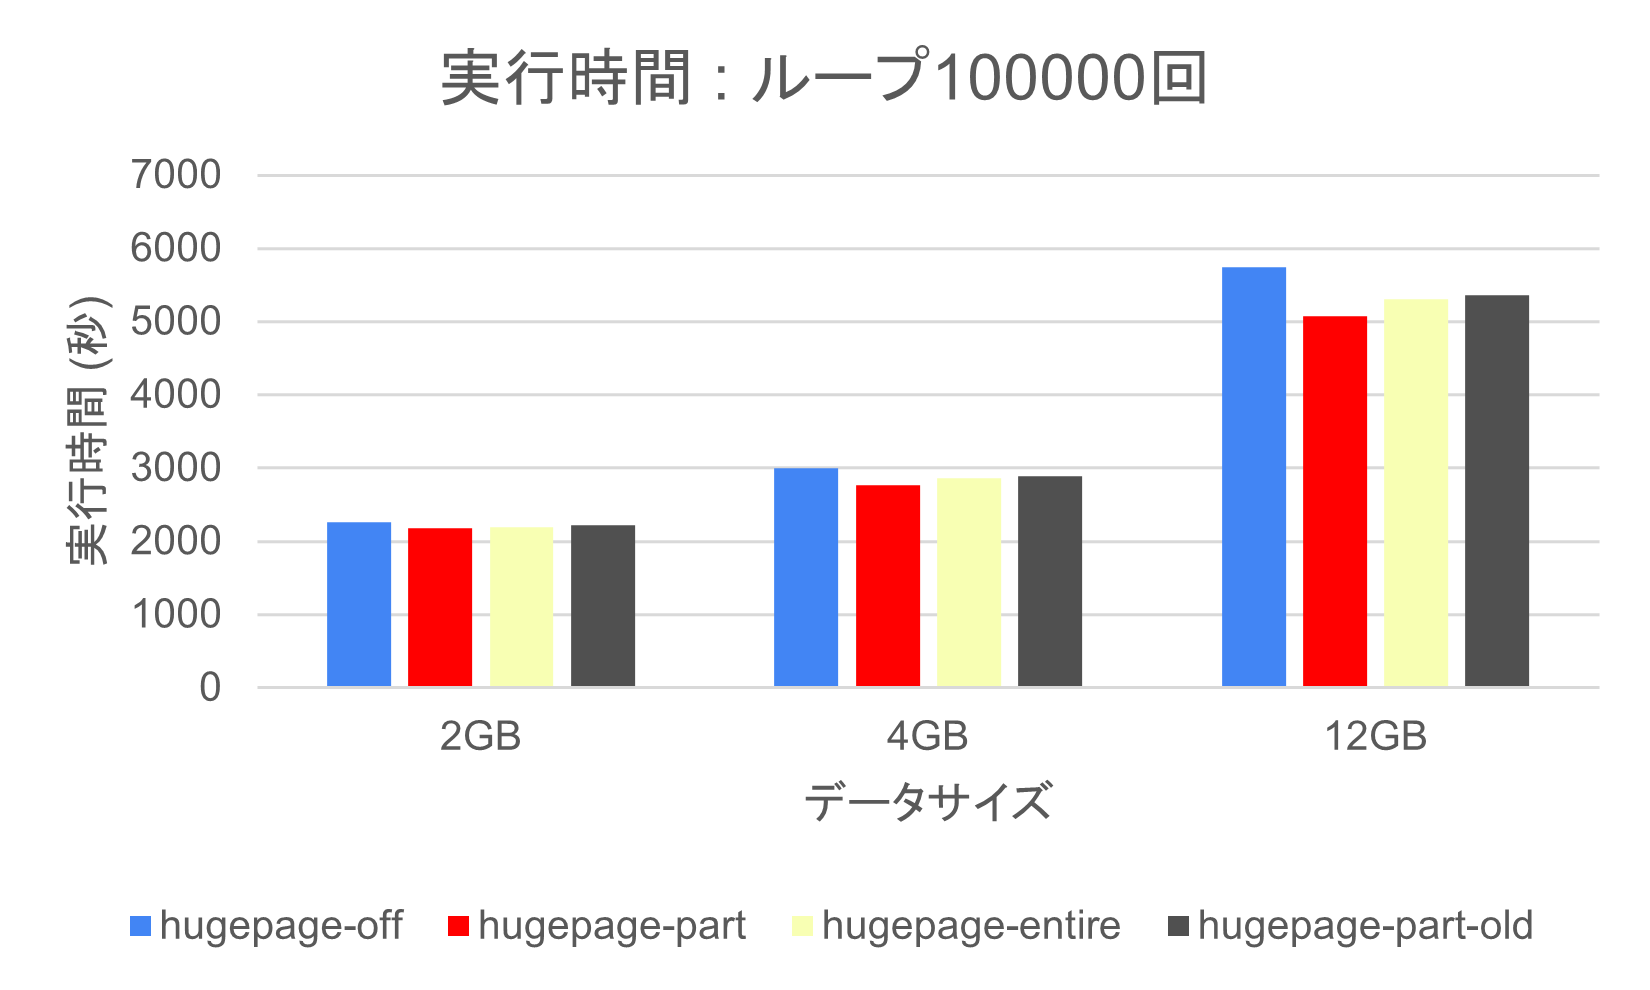
\includegraphics[scale=0.6]{figures/experiment-new/storagememory/exec-100000.png}
  \caption{実験結果:実行時間}
  \label{fig:storagememory-exec-100000}
\end{figure}

\subsection{TLBミス率}
TLBミス率を図\ref{fig:storagememory-tlb-miss-100000}に示す
全体割り当て,今回の提案方式が両方とも大きくTLBミス率を削減しており,このTLBミスの削減で実行時間が削減されたと分かる.
予備実験の手法は他よりも削減率が良くないことからヒュージページを使い始めるのが遅く恩恵を十分に受けられていないことが分かる.
対して今回の提案方式は全体割り当てに近く大幅なTLBミス率の削減ができているので,ヒュージページを最初から
十分に使えているとわかる.

\begin{figure}
  \centering
  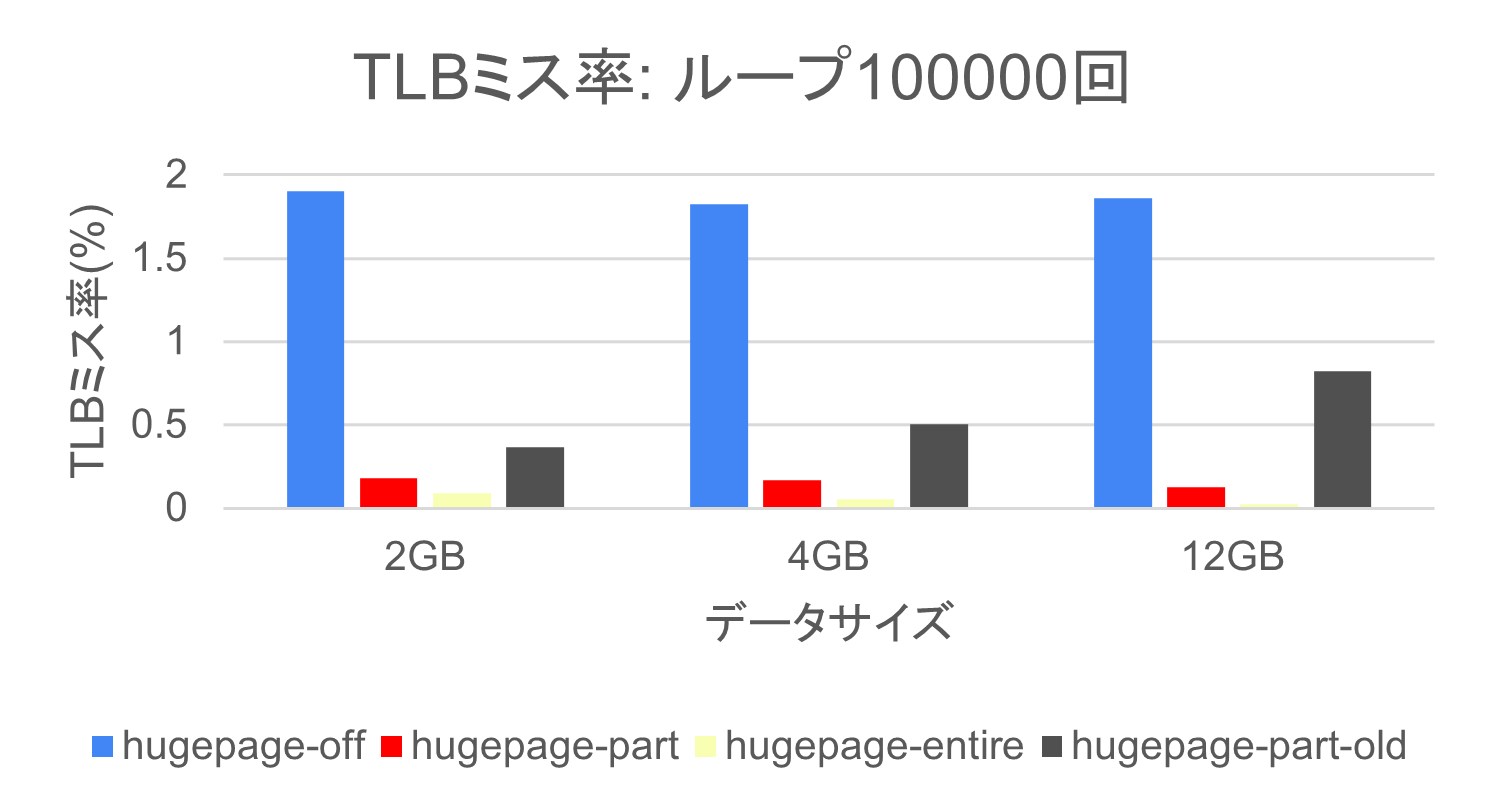
\includegraphics[scale=0.6]{figures/experiment-new/storagememory/tlb-miss-100000.png}
  \caption{実験結果:TLBミス率}
  \label{fig:storagememory-tlb-miss-100000}
\end{figure}

\subsection{ヒュージページ割り当て数の比較}
データサイズ12GBでのヒュージページ割り当て数の遷移を図\ref{fig:storagememory-throughput-hugepage-4g-100000}に示す.
今回の提案方式では即座に3GBの割り当てを行っている.サイズとして4つのExecutorが12GBをそれぞれ保存するため,
12/4 = 3GBのデータであり,StorageMemoryのデータをすぐに全部割り当てることができている.
予備実験の方式では割り当てに長い時間がかかっており,ヒュージページの恩恵を十全に受けられるまで時間が
かかっているのがわかる.
全体割り当てについてはStorageMemroy以外のデータにも割り当てを行っており,ヒュージページを使うサイズが
大きくなっている.この時の無駄な割り当てによるオーバーヘッドが実行時間に出てきていると考えられる.

\begin{figure}[H]
  \centering
  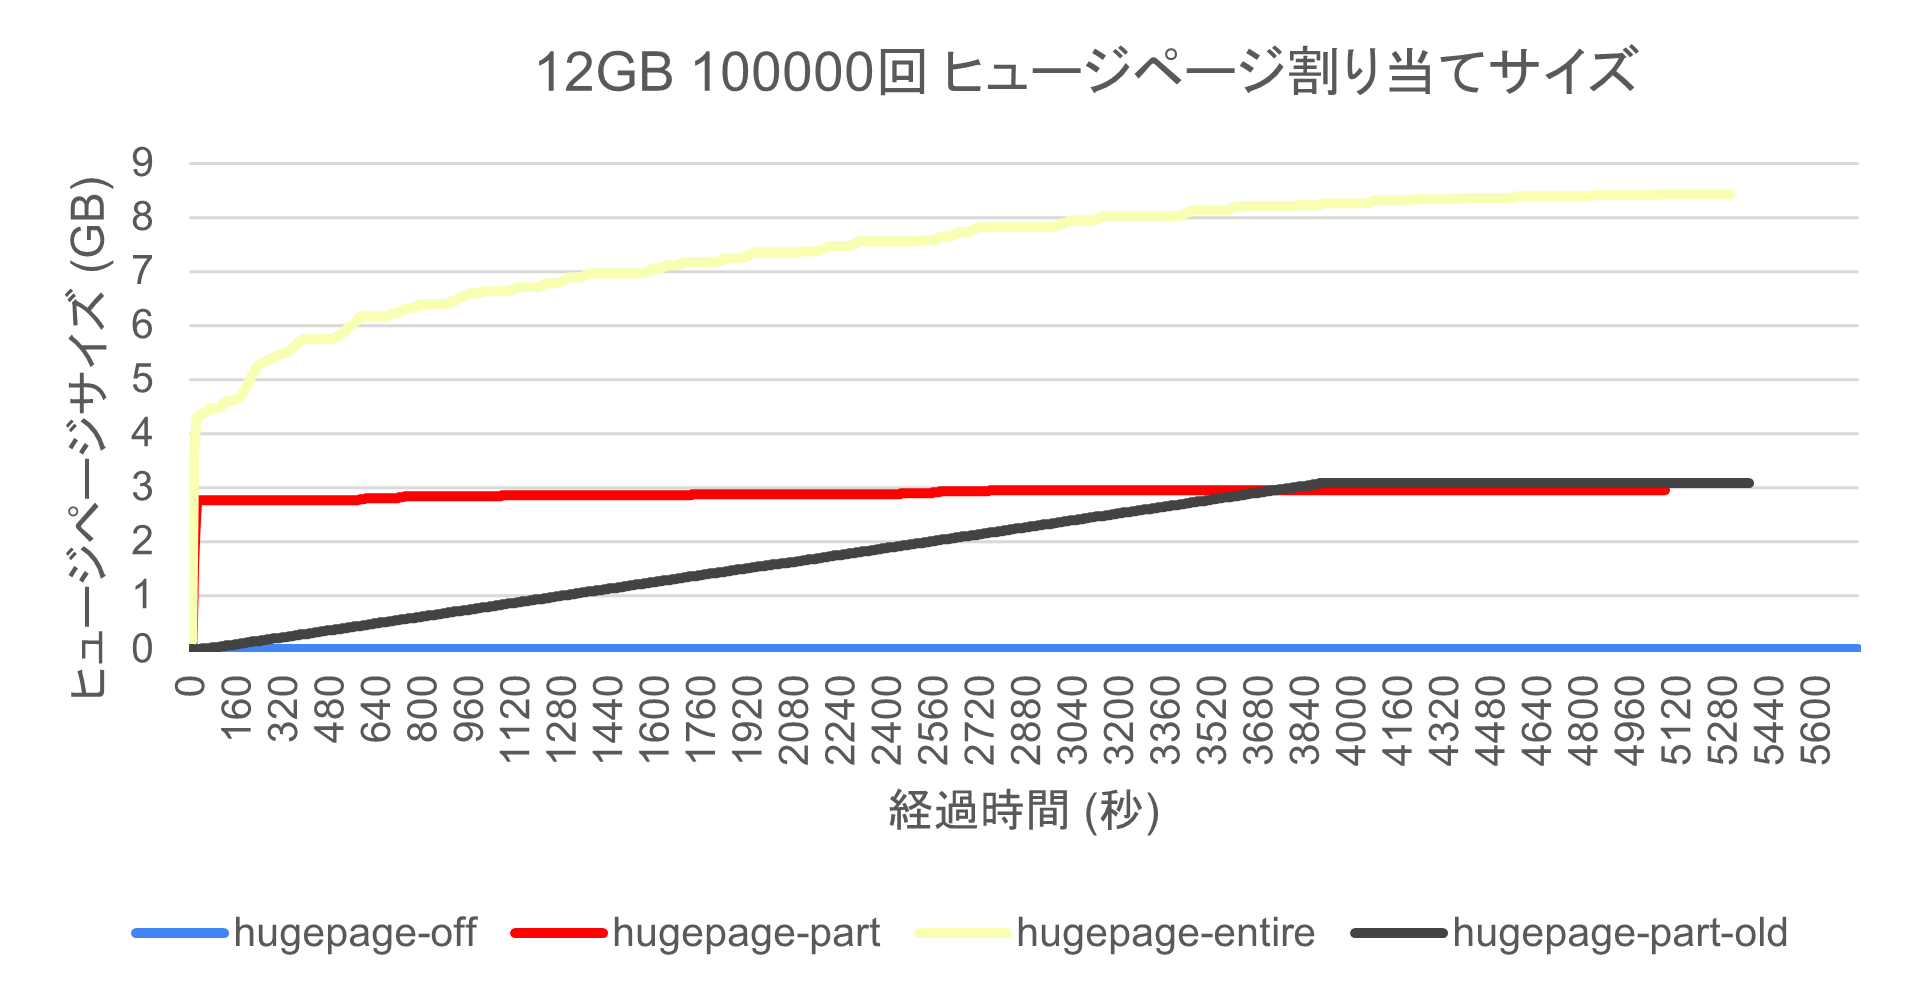
\includegraphics[scale=0.5]{figures/experiment-new/storagememory/throughput-hugepage-4g-100000.png}
  \caption{実験結果:ヒュージページ割り当てサイズ}
  \label{fig:storagememory-throughput-hugepage-4g-100000}
\end{figure}

\section{関連研究}
HotTub\cite{lion2016don}はJVMのウォームアップ時間を減らすことで分散処理フレームワークのパフォーマンスを向上させる
機構である.HotTubではJVMのウォームアップを減らすためにJVMの再利用を行う.一度使用したJVMは
通常そのまま終了されるところを一旦プールしておき,他のアプリケーションによってJVMを起動する時に
プールしておいたJVMを再利用することでウォームアップにかかる時間を短縮する.
結果としてHotTubはウォームアップ時間を短縮し,HDFS\cite{shvachko2010hadoop}の読み書きやSparkSQL\cite{armbrust2015spark}などのワークロードでの実行時間の
短縮に成功している.

Yak\cite{nguyen2016yak}は分散処理システムに適したGCで世代別GCと領域ベースのGCを組み合わせたものとなる.
YakではSparkのオブジェクト特性に注目し,オブジェクトが長寿でライフサイクルが同じであるという
ことを利用して,オブジェクト適正に合わせたGCを行うことでGC時間を短縮させている

Riffle\cite{zhang2018riffle}はMapReduceのシャッフルフェーズにオーバーヘッドが大きいことに注目し,シャッフルの際の
細かい中間データをマージして一つにすることでシャッフル時間を短縮させることに成功している.

Ingens\cite{kwon2016coordinated}はTHPの問題点を解決し効率的なヒュージページ管理を行う機構である.Ingensではヒュージページの
使用率とアクセス頻度を監視し,その情報をもとに適切なタイミングでヒュージページ割り当てを行うことで
断片化の解消やメモリの節約といったパフォーマンスの向上を行っている.

Illuminator\cite{panwar2018making}はTHPのメモリ汚染による断片化を減らし,効率的なヒュージページ管理を行う機構である.
IlluminatorではLinuxに存在するユーザ用の移動可能なmovableとカーネル用の移動不可能なunmvableな
メモリ領域に加えてmovableとunmovableが混在したハイブリッド領域を明示的に管理し,ハイブリッド
領域ではヒュージページ割り当てを避けることで無駄にページ移動することを防いでいる.
結果としてIlluminatorはページ移動にかかる時間を短縮させ,パフォーマンスを向上させている.

これらの研究はヒュージページと分散処理フレームワークそれぞれに個別に対処したものであり,
インメモリ分散処理フレームワークを対象としたヒュージページ割り当てに関する研究は行われていない.
本研究では分散処理フレームワーク固有の特性を考慮して効率的にヒュージページを利用する
手法を提案した.